\section{User Interface Prototypes}

The user interface for the mdrender shell application is very simple. A user will use the form "mdrender (flags) (filename)", and the program will output, as appropriate, an output file corresponding to the input file name entered by the user. Our UI mocks were created using a bash script that mocks the inputs and outputs of the fully featured program.

\subsection{Rendering markdown to PDF}

Because this is the default mode of the application, the user does not need to enter any flags to specify special behavior of the program; they simply run the command and are given an output file.

\noindent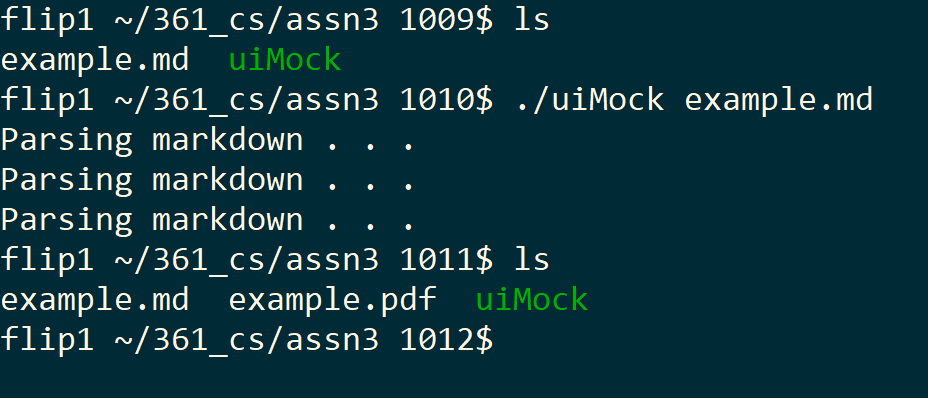
\includegraphics[width=350pt]{images/mdrender_pdf.png}

\subsection{Rendering markdown to HTML}

Similarly to rendering pdf files, the user will enter a command and find an output html file. To specify HTML as the output type, they add the "-h" flag for "html".

\noindent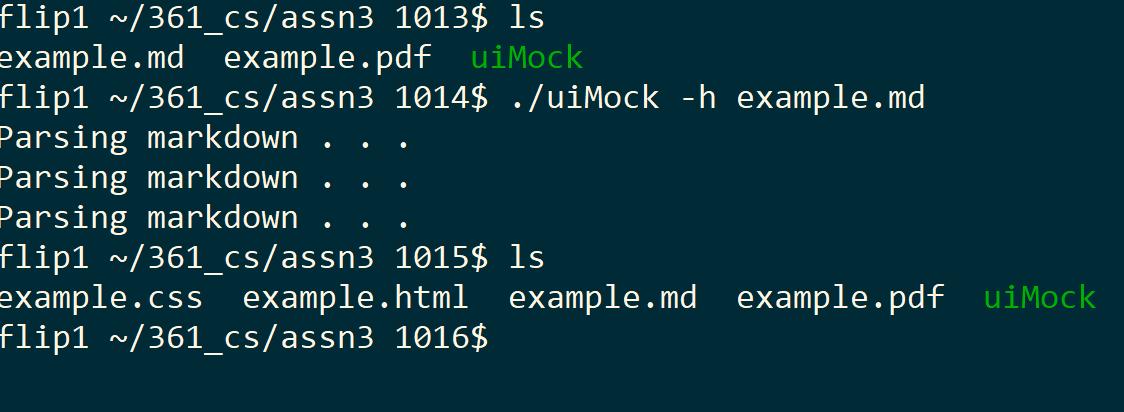
\includegraphics[width=350pt]{images/mdrender_html.png}
\subsection{Sending markdown data to STDOUT}

For this command, the user adds the "-d" flag, meaning "data" to the command. The program will output the parsed markdown to STDOUT instead of writing it to a file.

\noindent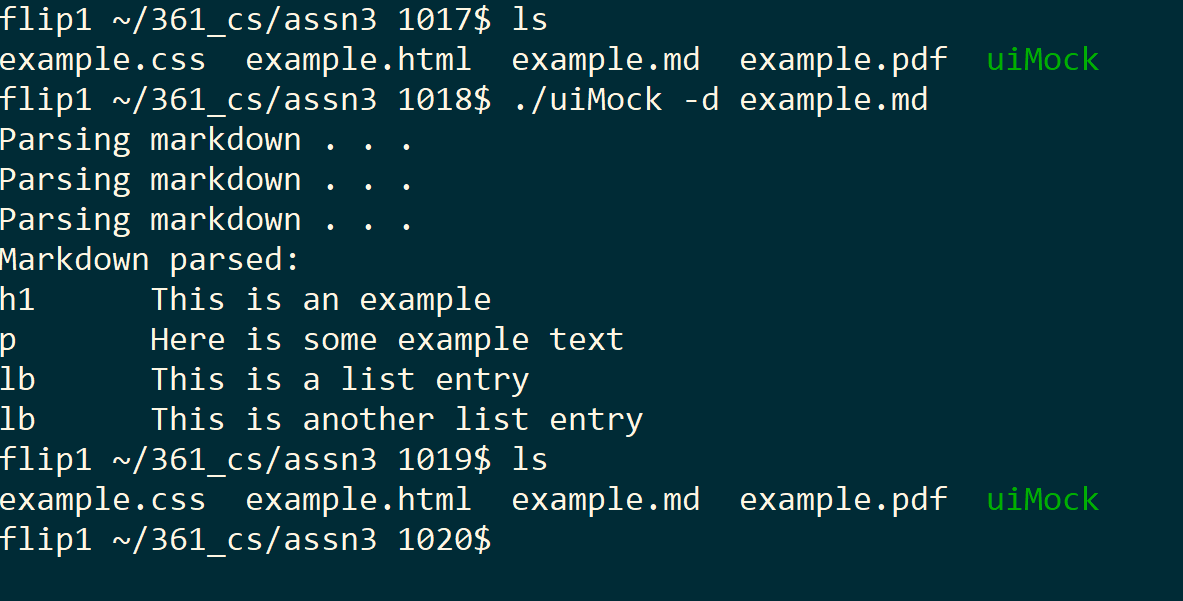
\includegraphics[width=350pt]{images/mdrender_stdout.png}
